\documentclass[a4paper]{article} 
\addtolength{\hoffset}{-2.25cm}
\addtolength{\textwidth}{4.5cm}
\addtolength{\voffset}{-3.25cm}
\addtolength{\textheight}{5cm}
\setlength{\parskip}{0pt}
\setlength{\parindent}{0in}

%----------------------------------------------------------------------------------------
%	PACKAGES AND OTHER DOCUMENT CONFIGURATIONS
%----------------------------------------------------------------------------------------

\usepackage{charter} % Use the Charter font
\usepackage[utf8]{inputenc} % Use UTF-8 encoding
\usepackage{microtype} % Slightly tweak font spacing for aesthetics
\usepackage{graphicx}
\usepackage[english]{babel} % Language hyphenation and typographical rules
\usepackage{amsthm, amsmath, amssymb} % Mathematical typesetting
\usepackage{float} % Improved interface for floating objects
\usepackage[final, colorlinks = true, 
            linkcolor = black, 
            citecolor = black]{hyperref} % For hyperlinks in the PDF
\usepackage{graphicx, multicol} % Enhanced support for graphics
\usepackage{xcolor} % Driver-independent color extensions
\usepackage{marvosym, wasysym} % More symbols
\usepackage{booktabs} % Enhances quality of tables
\usepackage[yyyymmdd]{datetime} % Uses YEAR-MONTH-DAY format for dates
\renewcommand{\dateseparator}{-} % Sets dateseparator to '-'
\usepackage{fancyhdr} % Headers and footers
\pagestyle{fancy} % All pages have headers and footers
\fancyhead{}\renewcommand{\headrulewidth}{0pt} % Blank out the default header
\fancyfoot[L]{} % Custom footer text
\fancyfoot[C]{\thepage} % Custom footer text
\fancyfoot[R]{} % Custom footer text

%----------------------------------------------------------------------------------------

\begin{document}

%-------------------------------
%	TITLE SECTION
%-------------------------------

\fancyhead[C]{}
\hrule \medskip % Upper rule
\begin{minipage}{0.295\textwidth} 
\raggedright
\footnotesize
Dylan Huber 
\end{minipage}
\begin{minipage}{0.4\textwidth} 
\centering 
\large 
DNA Extraction and PCR Write-up\\ 
\normalsize 
02-261\\ 
\end{minipage}
\begin{minipage}{0.295\textwidth} 
\raggedleft
\today\hfill\\
\end{minipage}
\medskip\hrule 
\bigskip

%-------------------------------
%	CONTENTS
%-------------------------------

\section{QC Results From DNA Extraction}

\begin{table}[h]
    \begin{center}
        \begin{tabular}{|c|c|c|c|c|}
            \hline 
            Sample ID & Nucleic Acid (ng/ul) & A260 (Abs) & A280 (Abs) & 260/280 \\
            \hline
            C4 & $1.0$ & $0.019$ & $0.011$ & $1.70$ \\
            C5 & $0.9$ & $0.017$ & $0.011$ & $1.63$ \\
            C12 & $2.1$ & $0.042$ & $0.009$ & $1.75$ \\
            \hline
        \end{tabular}
    \end{center}
    \caption{The QC results from my group's DNA extraction samples.}
\end{table}

\section{Gel Runs}

\begin{figure}[H]
    \centering
    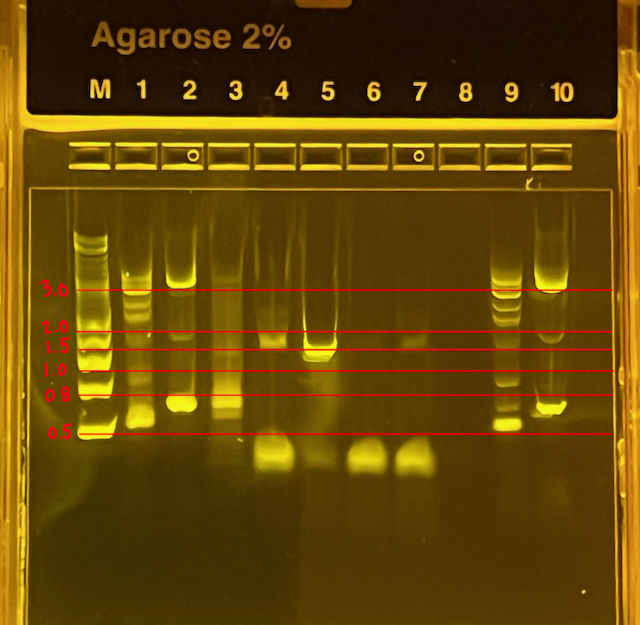
\includegraphics[width=0.75\linewidth]{IMG_9160.png}
    \caption{Our gel electrophoresis run. Number of bases marked along the ladder along lane M in red in kilobases. Contents of each lane are in the table below.}
\end{figure}

\begin{table}[h]
    \begin{center}
        \begin{tabular}{|c|c|c|}
            \hline 
            Lane Number & DNA & Primer\\
            \hline
            1 & C4 & Our Primer \\
            2 & C5 & Our Primer \\
            3 & C12 & Our Primer \\
            4 & C4 & Kangas Primer \\
            5 & C5 & Kangas Primer \\
            6 & C12 & Kangas Primer \\
            7 & None & Our Primer (Primer Control) \\
            8 & C4, C5, C12 & None (DNA Control) \\
            9 & C4 & Our Primer \\
            10 & C5 & Our Primer \\
            \hline
        \end{tabular}
    \end{center}
    \caption{The contents of each lane in the gel electrophoresis run.}
\end{table}

In lanes 1 and 2 (and their duplicates in lanes 9 and 10) we see good products that we wanted. This suggests that the primers we created did create a product in these samples. However, with the primer we added, we would expect a product of about $980$ bases, which is not what we see here (it looks to be about $600-700$ bases). This might be due to the primers bonding in incorrect places, or perhaps the sampled DNA is not one of the six that we tested upon.\\

In lane 3, we see a vague response at about $800$ bases as well. This is closer to what we wanted of $980$ bases. If this is the intended output that we wanted, this implies sample C12 had A1, A5, A6, or A7 within the sample (via our PCR lab).\\

Lanes 4 and 5 had good responses with the Kangas primer. This is good since it implies that there was indeed the correct type of DNA within the C4 and C5 samples.\\

Lane 6 doesn't seem to have much other than many really short DNA strands, which might be the primers. This somewhat weakens the idea that lane 3 had a true response, since if it did this lane would also be likely to have a response.\\

Lanes 7 and 8 are our controls and work as we would expect them to. We see the primers in the bottom of lane 7, and we see nothing in lane 8 since the DNA should be longer than anything on this scale.\\

\section{DNA Identification}

I looked specifically at the C5 sample. This DNA sample was IDed as the haemolyticus strain of Staphylococcus. My research led me to find that this is part of the ``skin flora'' of humans. I collected this sample from the handle of a doorway into a section of Wean Hall. Thus, having a strain of bacteria from human skins makes a lot of sense.

\section{Conclusions}

In conclusion, I believe we did quite well with extracting the DNA. Our sample was pure enough that the identification company found a strong match for the bacteria. Additionally, we had PCR results for many of our extractions, which means that they did indeed have DNA in them.\\

On the other hand, our primers did not quite work as intended. As mentioned earlier the length of the products were not as expected. This error could have been caused by incorrect selection of primers, a poor gel run which skewed the read lengths, or a corruption of the DNA contents, which caused the primers to react with some other DNA that made products of the length observed.

\end{document}